%!TEX root = ../thesis.tex

\section{背景}
農林水産省 \cite{farmer} によると, 日本の農業従事者数は, 2000年から2023年にかけて約50%減少している.
また, 2023年の農業従事者のうち約7割が65歳以上の高齢者となっている.
そのため, 日本の農業分野では人手不足と高齢化による農作業の負担増大が深刻な問題となってきている.
これらの問題を解決するために作物を自動で収穫することができるロボットの開発が望まれる.
収穫ロボットに求められる技術のうちの1つに収穫用のエンドエフェクタが挙げられる.

\vspace{5mm}

現在, 収穫用エンドエフェクタに関する研究は多く, 既に様々なエンドエフェクタが提案されている.
例えば, Bacらはピーマン収穫ロボットを開発し, 2種類のエンドエフェクタを提案している \cite{finray}.
1つがフィンレイエンドエフェクタであり, グリッパで果実を把持して, ハサミで花柄を切断するものである.
グリッパにはフィンレイ効果が利用されていて, 果実を包み込むように把持することができる.
もう1つがリップ型エンドエフェクタであり, 吸着パッドで果実を把持して, 唇のような形の刃で花柄を切断し収穫する.

\begin{figure}[H]
     \centering
     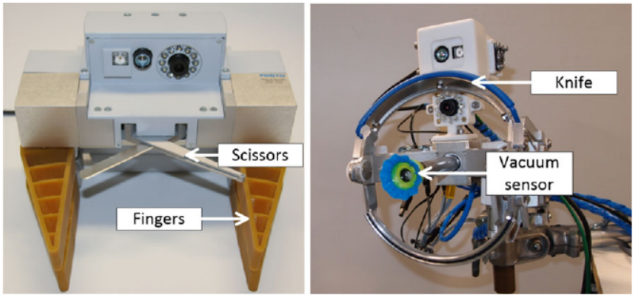
\includegraphics[width=130mm]{images/png/finray.png}
     \caption{Fin Ray end effector (left) and Lip-type end effector (right)}
     \label{Fig:finray}
   \end{figure}

また, Aradらは「SWEEPER」と呼ばれるピーマン収穫ロボットを開発し, 振動ナイフを用いて収穫するエンドエフェクタを提案している \cite{sweeper}.
こちらは刃を振動させて花柄を切断し, エンドエフェクタの下部についた指のようなもので果実をキャッチしている.
このエンドエフェクタは果実を把持しないため, 把持によってピーマンに傷がつくことはない.

\vspace{5mm}
\begin{figure}[H]
     \centering
     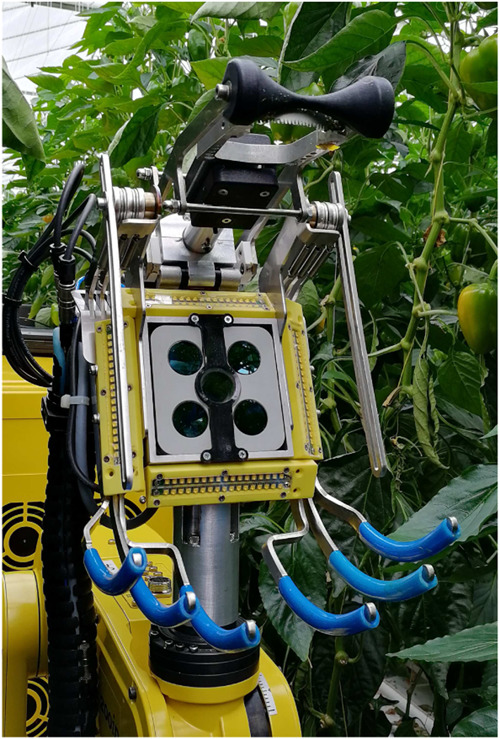
\includegraphics[width=50mm]{images/png/sweeper.png}
     \caption{vibrating knife end effector}
     \label{Fig:sweeper}
   \end{figure}

論文で提案されているもの以外にも, 市販されている収穫ロボットに独自のエンドエフェクタが取り付けられているものもある.
AGRISTが開発した「L」という収穫ロボットに搭載されているエンドエフェクタは, 花柄に直接アプローチしてピーマンを収穫する \cite{agrist}.
花柄を切断後, そのまま花柄を把持して収穫するので, 果実を傷つける心配がなく, 花柄さえ見れていれば収穫することができる.

\vspace{5mm}
\begin{figure}[H]
     \centering
     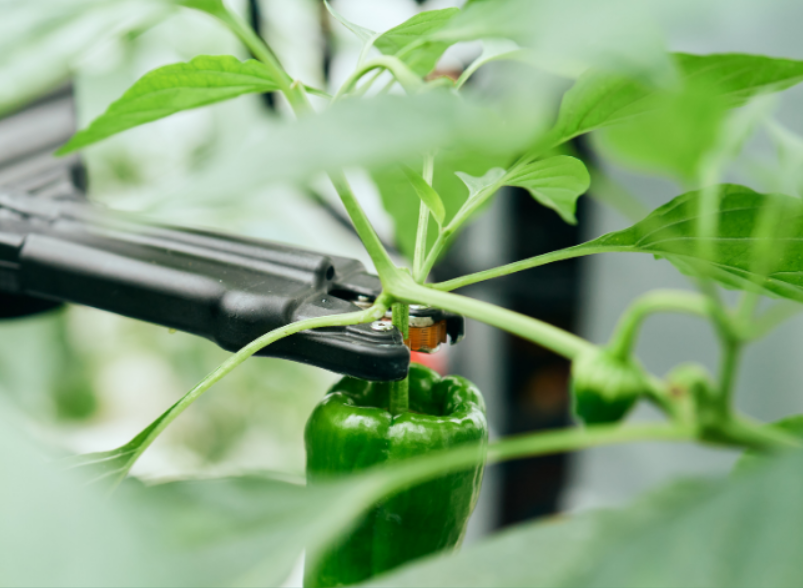
\includegraphics[width=100mm]{images/png/agrist.png}
     \caption{End effector that directly approaches the peduncle}
     \label{Fig:agrist}
   \end{figure}

しかし, それらのエンドエフェクタの設計指針については明確に示されていない.
そのため, 収穫する作物に対して優れた形状がわからないことや, 具体的な改善点が見つけにくいことが問題となる.

\vspace{5mm}

Fig.?のような場合において, 赤で示されたピーマンは花柄が露出しているが果実は葉で隠れてしまっているのに対し, オレンジで示されたピーマンは花柄が葉で隠れているが果実は露出している.
赤で示されたピーマンは花柄にアプローチしやすく, AGRISTの「L」に搭載されている花柄に直接アプローチするタイプのエンドエフェクタが適していると考えられる.
一方でオレンジで示されたピーマンは果実にアプローチしたほうがよく, 果実を掴んで引っ張るなどの方法で収穫するエンドエフェクタが良いのではないかと予想できる.
このことから, 収穫物のいくつかの特性を定量化することで収穫物に適したエンドエフェクタの形を考える.

\vspace{5mm}
\begin{figure}[H]
     \centering
     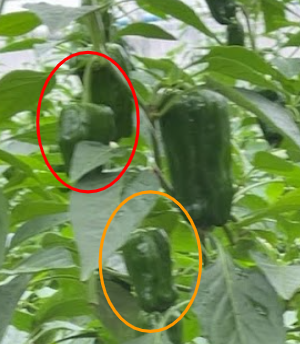
\includegraphics[width=100mm]{images/png/plantex.png}
     \caption{Example green pepper plant}
     \label{Fig:plantex}
   \end{figure}

% \subsection{RoboCup}

% \begin{figure}[hbtp]
%   \centering
%  \includegraphics[keepaspectratio, scale=0.8]
%       {images/RaspberryPiMouse.png}
%  \caption{Example}
%  \label{Fig:Example}
% \end{figure}

% \subsubsection{etc...}
\newpage
